\documentclass{beamer}

\usepackage{amsmath}
\usepackage[style=alphabetic,url=true]{biblatex}
\usepackage{environ}
\usepackage{geometry}
\usepackage{graphicx}
\usepackage{amsmath}
\usepackage{amsfonts}
\usepackage{amssymb}
\usepackage{calrsfs}
\usepackage{listings}
\usepackage{tikz}
\usepackage[T2A]{fontenc}
\usepackage[utf8]{inputenc}
\usepackage[cache=false]{minted}

\graphicspath{ {./graphics/} }
\usetikzlibrary{shapes.arrows,chains}
\usecolortheme{beaver}
\setbeamertemplate{itemize item}[circle]
\setbeamertemplate{itemize subitem}{--}
\addtobeamertemplate{navigation symbols}{}{
  \usebeamerfont{footline}
  \usebeamercolor[fg]{footline}
  \hspace{1em}
  \insertframenumber/\inserttotalframenumber
}
\setminted[Lisp]{
  fontsize=\footnotesize
}
\BeforeBeginEnvironment{minted}{\medskip}
\AfterEndEnvironment{minted}{\medskip}



\title{
  Common Lisp and Introduction to Functional Programming \\
  Lecture 2: Common Lisp Basics
}
\author{Yuri Zhykin}
\date{Feb 11, 2021}

\begin{document}

\frame{\titlepage}

\begin{frame}
  \frametitle{$\lambda$-calculus 1/2}
  \begin{itemize}
  \item Introduced by Alonzo Church in 1930s.
  \item $\lambda$-calculus is a formal system in mathematical logic for
    expressing computation based on function abstraction and application using
    \textbf{variable binding} and \textbf{substitution}.
  \item Church showed that all \textit{computable} functions can be expressed in
    $\lambda$-calculus.
  \item Church and Turing showed that \textit{Turing machine model} and
    \textit{$\lambda$-calculus} are equivalent.
  \end{itemize}
\end{frame}

\begin{frame}
  \frametitle{$\lambda$-calculus 2/2}
  \begin{itemize}
  \item Primitives:
    \begin{itemize}
    \item $x$ - \textbf{variable} - a symbol representing a parameter or value.
    \item $(\lambda x . M)$ - \textbf{abstraction} - function definition; $M$ is a
      \textit{$\lambda$-term}.
    \item $(M\;N)$ - \textbf{application} - applying a function to an argument;
      both $M$ and $N$ are \textit{$\lambda$-terms}.
    \end{itemize}
  \item Operations:
    \begin{itemize}
    \item $(\lambda x . M[x]) \rightarrow (\lambda y . M[y])$ -
      \textbf{$\alpha$-reduction} - renaming a variable to avoid name
      collisions.
    \item $((\lambda x . M) E) \rightarrow (M[x := E])$ -
      \textbf{$\beta$-reduction} - replacing variable with the argument
      expression (calculation step).
    \item $f \leftrightarrow \lambda x . (f\;x)$ -
      \textbf{$\eta$-reduction} - drop an \textit{abstraction} for simplicity.
    \end{itemize}
  \item Example: $((\lambda x\;.\;2 \cdot x)\;12) \rightarrow (2 \cdot 12)
    \rightarrow 24$
  \end{itemize}
\end{frame}

\begin{frame}
  \frametitle{$\lambda$-calculus and Lisp History}
  \begin{itemize}
  \item John McCarthy - Recursive Functions of Symbolic Expressions and Their
    Computation by Machine, Part I, 1958-1960.
  \item Steve Russel implemented the evaluator for the LISP (LISt Processing)
    system in machine code for \textbf{IBM 704} machine.
  \item M-expressions ($f[g[A,B]]$) and $S$-expressions ($(f (g A B))$).
  \item First complete LISP compiler (Tim Hart, 1962) introduced incremental
    compilation.
  \item Dozens of dialects; modern ones include:
    \begin{itemize}
    \item Common Lisp
    \item Emacs Lisp
    \item Clojure
    \item Scheme (Racket)
    \end{itemize}
  \end{itemize}
\end{frame}

\begin{frame}
  \frametitle{Syntax 1/2}
  \begin{itemize}
  \item Polish notation: operator (function name) prefixes the operands;
    eliminates operator precedence rules:
    \begin{itemize}
    \item \mintinline{Lisp}{2 * x + y}
    \item \mintinline{Lisp}{(+ (* 2 x) y)}
    \end{itemize}
  \item Whole syntax consists of S-expressions and closely follows
    $\lambda$-calculus notation:
    \begin{itemize}
    \item $((\lambda x\;.\;2 \cdot x)\;12)$
    \item \mintinline{Lisp}{((lambda (x) (* 2 x)) 12)}
    \end{itemize}
  \item Lisp expressions can be of two types:
    \begin{itemize}
    \item \textbf{atoms} evaluate to the values they denote,
    \item \textbf{lists} evaluate as
      \mintinline{Lisp}{(<operator> <operand1> <operand2> ...)},
      except if they denote \textit{special forms}.
    \end{itemize}
  \end{itemize}
\end{frame}

\begin{frame}[fragile]
  \frametitle{Syntax 2/2}
  \begin{itemize}
  \item Lisp expressions are trees of atoms \mintinline{Lisp}{(- (* 2 (+ 14 7) 6))}
    \begin{center}
      \begin{tikzpicture}[->] 
        \node {-}
        child{ node {*}
        child{ node {2} }
        child{ node {+}
          child{ node {14} }
          child{ node {7} }}
        child{ node {6}}};
      \end{tikzpicture}
    \end{center}
  \end{itemize}
\end{frame}

\begin{frame}[fragile]
  \frametitle{Lisp REPL 1/2}
  \begin{itemize}
  \item \textbf{Read Eval Print Loop} - Lisp expression is read, evaluated, and
    the result is printed for the user to see. 
  \item Literal evaluation:
\begin{minted}{Lisp}
  CL-USER> "Hello, World!"
  "Hello, World!"
  CL-USER> 1000000
  1000000
\end{minted}
  \item Function evaluation:
\begin{minted}{Lisp}
  CL-USER> (* 2 (+ 14 7))
  42
  CL-USER> (print "Hello, World!")
  Hello, World!
  "Hello, World!"
\end{minted}
  \end{itemize}
\end{frame}

\begin{frame}[fragile]
  \frametitle{Lisp REPL 2/2}
  \begin{itemize}
  \item Lisp has built-in variables to access evaluation history:
\begin{minted}{Lisp}
  CL-USER> (+ 1 2)
  3
  CL-USER> (+ * 3)
  6
  CL-USER> (+ * 4)
  10
  CL-USER> (* ** ***) ;; (* 6 3)
  18
\end{minted}    
  \end{itemize}
\end{frame}

\begin{frame}[fragile]
  \frametitle{Data Structures: Pairs}
  \begin{itemize}
  \item \mintinline{Lisp}{nil} - a constant value that represents nothing (Latin \textit{nihil}).
  \item \textit{Pair} - a combination of two values (a.k.a. \textit{cons-cell}):
\begin{minted}{Lisp}
  CL-USER> (cons 1 2)
  (1 . 2)
  CL-USER> (car (cons 1 2))
  1
  CL-USER> (cdr (cons 1 2))
  2
\end{minted}
  \item Pairs can contain any values:
\begin{minted}{Lisp}
  CL-USER> (cons "John" 9000)
  ("John" . 9000)
  CL-USER> (cons 1 nil)
  (1)
\end{minted}
  \end{itemize}
\end{frame}

\begin{frame}[fragile]
  \frametitle{Data Structures: Lists 1/2}
  \begin{itemize}
  \item \textit{Singly linked list}, or just \textit{list}:
\begin{minted}{Lisp}
  CL-USER> (cons 1 (cons 2 (cons 3 (cons "John" nil))))
  (1 2 3 "John")
  CL-USER> (list 1 2 3 "John")
  (1 2 3 "John")
\end{minted}
  \item Proper lists always have \mintinline{Lisp}{nil} as
    \mintinline{Lisp}{cdr} of the innermost \mintinline{Lisp}{cons}:
\begin{minted}{Lisp}
  CL-USER> (cons 1 (cons 2 (cons 3 "John")))
  (1 2 3 . "John")
\end{minted}
  \item \mintinline{Lisp}{nil} also denotes an empty list:
\begin{minted}{Lisp}
  CL-USER> (list)
  nil
\end{minted}
  \end{itemize}
\end{frame}

\begin{frame}[fragile]
  \frametitle{Data Structures: Lists 2/2}
  \begin{itemize}
  \item \textbf{Head} and \textbf{tail} of a list can be accessed with the
    \mintinline{Lisp}{car} and \mintinline{Lisp}{cdr} function:
\begin{minted}{Lisp}
  CL-USER> (car (list 1 2 3)) ;; (car (cons 1 (cons 2 ...)))
  1
  CL-USER> (cdr (list 1 2 3)) ;; (cdr (cons 1 (cons 2 ...)))
  (2 3 "John")
\end{minted}
  \end{itemize}
  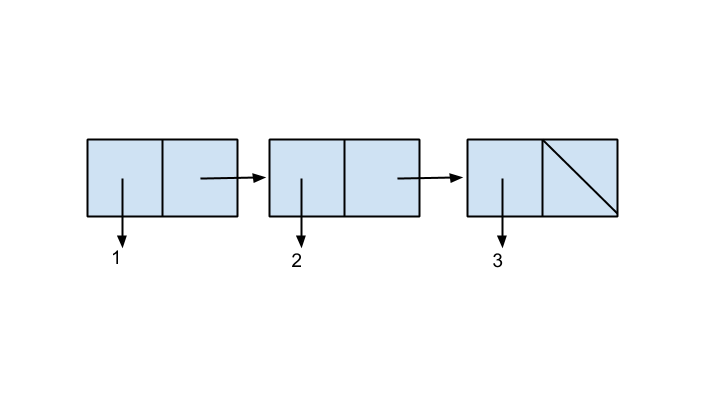
\includegraphics[width=\columnwidth,trim={0 1cm 0 1cm},clip]{box-and-pointer}
\end{frame}

\begin{frame}[fragile]
  \frametitle{Quoting}
  \begin{itemize}
  \item Lisp expressions can be ``quoted'' - the evaluation rules will not by
    applied to them:
\begin{minted}{Lisp}
  CL-USER> (quote (+ 1 2))
  (+ 1 2)
  CL-USER> '(+ 1 2)
  (+ 1 2)
\end{minted}
  \item List of \textit{atoms} that represents a Lisp expression can be
    evaluated with the \mintinline{Lisp}{eval} function:
\begin{minted}{Lisp}
  CL-USER> (eval '(+ 1 2))
  3
\end{minted}
  \end{itemize}
\end{frame}

\begin{frame}[fragile]
  \frametitle{Symbols 1/2}
  \begin{itemize}
  \item What exactly are atoms that are not literals?
\begin{minted}{Lisp}
  CL-USER> (type-of (car '(cons 1 2)))
  symbol
\end{minted}
  \item Symbol is a core data structure of a Lisp system.
  \item Symbols represent names within a Lisp system and are grouped into
    \textit{packages}.
  \item Symbol object contains 3 main fields:
    \begin{itemize}
    \item \mintinline{Lisp}{symbol-name},
    \item \mintinline{Lisp}{symbol-value},
    \item \mintinline{Lisp}{symbol-function},
    \end{itemize}
  \end{itemize}
\end{frame}

\begin{frame}[fragile]
  \frametitle{Symbols 2/2}
  \begin{itemize}
  \item When non-atomic Lisp expression is evaluated, the function is retrieved
    from the \mintinline{Lisp}{function} field of the symbol in the head of the
    list.
  \item Lisp languages that separate \mintinline{Lisp}{symbol-value} from
    \mintinline{Lisp}{symbol-function} are called Lisp-2 languages, as opposed
    to Lisp-1 languages that have a single namespaces for symbol values and
    symbol functions.
  \item In Lisp-2 languages, the function that will be called in each
    expression of the form
\begin{minted}{Lisp}
  (<function> <argument1> <argument2> ...)
\end{minted}
    is known at compilation time, which allows compilers to generate very
    efficient machine code.
  \end{itemize}
\end{frame}

\begin{frame}
  \frametitle{Lisp Development Environment}
  \begin{itemize}
  \item \textbf{SBCL}/\textbf{Allegro CL} - Lisp implementation (compiler and
    interpreter).
  \item \textbf{Emacs} - extensible text editor written in C and Emacs Lisp;
    around since 1976; approximately 5000 packages available.
  \item \textbf{SLIME} - Emacs package that provides Lisp IDE functionality
    (REPL, cross-reference, selective compilation in source files, etc).
  \item \textbf{Paredit} - Emacs package that provides structural editing
    capabilities (operate on whole S-expressions instead of characters).
  \end{itemize}
\end{frame}

\begin{frame}
  \frametitle{Emacs + SLIME}
  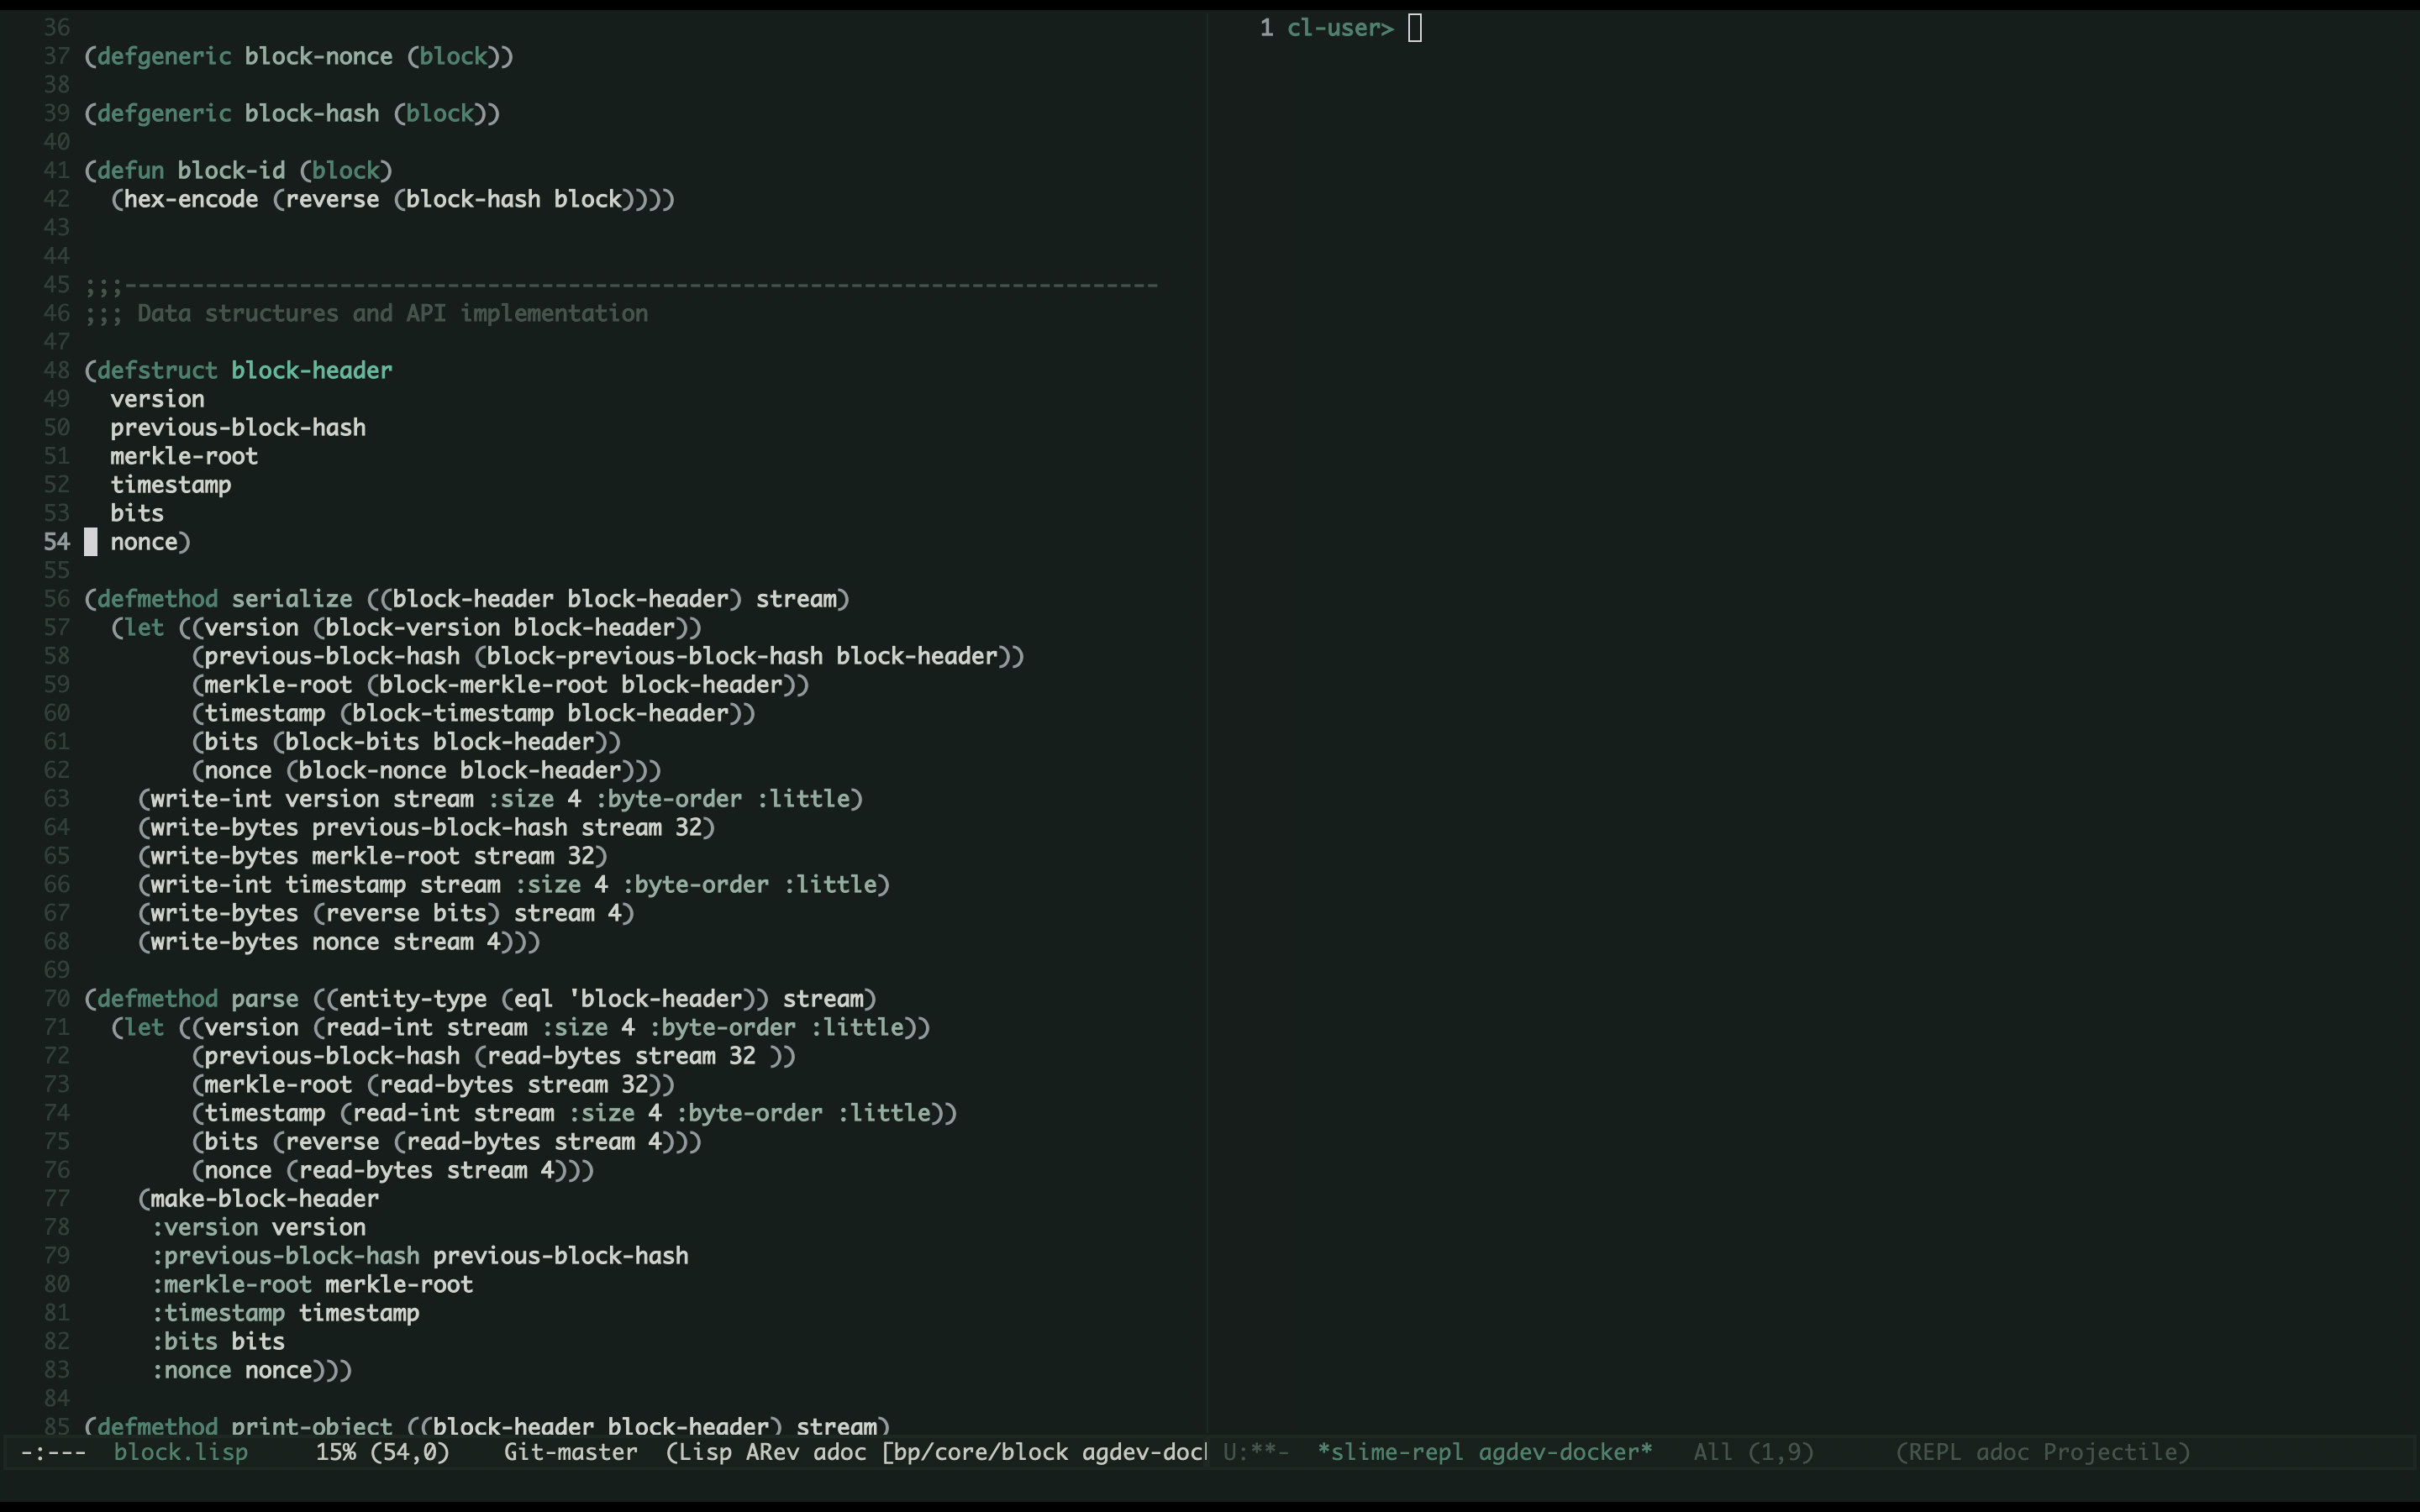
\includegraphics[width=\columnwidth]{emacs-lisp-ide}
\end{frame}

\begin{frame}
  \frametitle{The End}
  \begin{center}
    Thank you!
  \end{center}
\end{frame}

\end{document}

%%% Local Variables:
%%% mode: latex
%%% TeX-master: t
%%% TeX-command-extra-options: "-shell-escape"
%%% End:
